% ECON 691H Assignment 4: Data Description (due 2026-09-30).
% Figures and tables are produced by notebooks/descriptive_figures.ipynb; re-run it before compiling.
\documentclass[11pt]{article}

\usepackage[margin=1in]{geometry}
\usepackage[T1]{fontenc}
\usepackage{newtxtext,newtxmath}   % Times, matching the figure typeface
\usepackage{amsmath}
\usepackage{graphicx}
\usepackage{booktabs}
\usepackage{float}
\usepackage[font=small,labelfont=bf,labelsep=period,justification=justified,singlelinecheck=false]{caption}
\usepackage[authoryear,round]{natbib}
\usepackage[hidelinks]{hyperref}

\graphicspath{{../output/figures/}}
\newcommand{\tablepath}{../output/tables}
\setlength{\parskip}{0.4em}

\title{Who Bears the Shock? Bank Size and the Cross-Sectional\\
       Distribution of Bank Outcomes over the Business Cycle}
\author{William Rouse\\ \small ECON 691H: Data Description}
\date{September 30, 2026}

\begin{document}
\maketitle

\begin{abstract}
\noindent
Most evidence on how banks respond to macroeconomic shocks describes the average bank or the industry aggregate. This project instead asks how the entire cross-sectional distribution of bank outcomes (its location, spread, and asymmetry) shifts with the business cycle, and whether that response differs between the largest institutions and everyone else. Using the universe of FDIC-insured institutions from 1992 to 2026, I measure one-, two-, and three-quarter growth in total assets, the main outcome, alongside changes in capital, profitability, and net interest margin, and document how the quantiles of these changes move in expansions and recessions. Preliminary evidence shows that dispersion widens in recessions for every outcome, that the downside tails of profitability and capital lengthen sharply in the 2008--09 crisis, and that the largest banks have markedly more right-skewed asset growth.
\end{abstract}

\section*{Data Source}

The main data source is the Federal Deposit Insurance Corporation's \emph{BankFind Suite}, available through the public \href{https://banks.data.fdic.gov/bankfind-suite/bulkData/bulkDataDownload}{FDIC Website}. The BankFind Suite is compiled by the FDIC from the quarterly Consolidated Reports of Condition and Income (``call reports'') that every insured commercial bank and savings institution must file with its federal regulator, supplemented by FDIC structure data on charter type, regulator, and location. Because filing is mandatory, the data are a census rather than a sample: each quarter covers every FDIC-insured institution, from about 14{,}400 in 1992Q1 to about 4{,}200 in 2026Q2. I downloaded all 138 quarterly files from 1992Q1 through 2026Q2, each with 161 variables covering the balance sheet, the income statement, and precomputed performance ratios. Stacked, they form an unbalanced panel whose unit of observation is the bank-quarter, with institutions identified across time by their FDIC certificate number.

Census coverage over a long quarterly panel is what makes the data suited to this question. Studying the tails of a distribution requires many observations per period, and BankFind Suite supplies thousands of banks in every quarter across the 2001, 2007--09, and 2020 recessions. Holding-company data (FR Y-9C) and market data cover only large or listed organizations, so neither can describe the small, privately held community banks that make up nearly all institutions. Documentation is good but scattered: the BankFind data dictionary defines each variable, but the dictionary does not always say whether a ratio is year-to-date or quarterly, a distinction that turns out to be critical below. I add real GDP (FRED series GDPC1) and the NBER business-cycle chronology to classify quarters as recession or expansion.

\section*{Constructing the Analysis Dataset}

The 138 quarterly files are stacked into one bank-quarter panel keyed by certificate number and report date. I verify the merge by checking that the row counts agree and by comparing 6{,}900 randomly drawn cells against the raw files, all of which match. Three construction steps shape the analysis. First, I exclude insured U.S.\ branches of foreign banks (charter class OI; 40 institutions and 2{,}069 bank-quarters). These branches report assets but no equity or income, and the FDIC records their ROA and NIM as placeholder zeros that would otherwise enter the distributions as spurious zero changes. Second, because the FDIC reports ROA and NIM year-to-date and annualized, I recover each bank's single-quarter ratio as $r^{q}_{Q} = Q\, r^{\mathrm{ytd}}_{Q} - (Q-1)\, r^{\mathrm{ytd}}_{Q-1}$ within each calendar year, so that first-quarter values are not compared with full-year values. Third, I rank banks by total assets within each quarter and assign the top 1 percent (42 to 143 institutions depending on the year) to a large-bank group and the remainder to an other-bank group, re-assigning membership every quarter. For each horizon $k\in\{1,2,3\}$, I match each bank to its own record $k$ quarters earlier and compute the percent change in total assets (dollar changes are not comparable across banks that differ in size by orders of magnitude) and the percentage-point changes in the equity-to-assets ratio, ROA, and NIM.

\section*{Estimation Sample}

After the foreign-branch exclusion, the starting sample contains 1{,}127{,}856 bank-quarters from 17{,}121 institutions. No observations have missing or nonpositive assets, and none have missing ROA, NIM, or equity. A change can be computed only when the same institution reports in both $t-k$ and $t$, so the one-quarter estimation sample for asset growth contains 1{,}110{,}723 bank-quarters (11{,}057 in the large-bank group) covering 1992Q2--2026Q2, with 1{,}093{,}819 and 1{,}077{,}087 observations at $k=2$ and $k=3$. The same sample applies to the equity ratio; the ROA and NIM samples are 2{,}112 observations smaller because a bank's single-quarter ratio cannot be recovered when its previous same-year filing is missing.

Requiring consecutive filings makes the sample selective in the lower tail. Banks that fail or are absorbed drop out after their last call report, so their worst quarter can be missing, and this attrition is concentrated in 2008--10, so the sample probably understates how far the crisis downside tail stretched. The size grouping raises a second issue: because membership uses assets at $t$, a bank that entered the top 1 percent through rapid growth or an acquisition is mechanically a large bank with a large asset change, inflating the large-bank upper tail. Grouping on assets at $t-k$ is a planned robustness check. The large-bank group is also small, so its 10th and 90th percentiles rest on the 4th to 14th most extreme institution; for estimation I expect to widen the cutoff to the top 5 or 10 percent.

\section*{Key Variable: Asset Growth}

My main dependent variable is the growth rate of a bank's total assets. It measures the quantity side of a bank's response to a shock: how far the institution expands or contracts its balance sheet, and therefore its capacity to lend, hold securities, and take deposits. Total assets (column header: ASSET) are reported on the call-report balance sheet as the end-of-quarter book value in thousands of nominal dollars. For bank $i$ and horizon $k\in\{1,2,3\}$ I define
\[
  g^{(k)}_{it} = 100 \times \left( A_{it} / A_{i,t-k} - 1 \right),
\]
the percent change from the same bank's filing $k$ quarters earlier. Every bank in the sample reports positive assets, so the measure is defined whenever both filings exist and has no placeholder values.

The construction involves three choices. First, I use growth rates rather than dollar changes, because the largest banks are several orders of magnitude bigger than the median bank. Second, I leave assets in nominal terms. Deflating would subtract the same inflation rate from every bank in a quarter, so it would shift the location of each quarter's distribution without changing its spread or skewness, which are the objects of interest. It does mean that median growth in high-inflation years such as 2021--22 is not directly comparable to other years. Third, I use simple percent changes rather than log differences. Percent changes are bounded below at $-100$ and unbounded above, which mechanically adds right skew; log growth is a natural robustness check. The main alternatives are loan growth, the usual quantity measure in the bank lending channel literature, and deposit growth. I prefer total assets as the headline measure because it covers the whole balance sheet, including the securities that banks buy when loan demand falls, and is comparable across business models. Loan and deposit growth are constructed in the same way and used as companion outcomes. 

The main limitation is that reported assets include inorganic growth. An acquisition shows up as a large one-quarter jump for the acquirer, and the target disappears from the sample, so merger activity inflates the upper tail, especially for large banks in the consolidation wave of the late 1990s. A planned construction step is to flag structure-change quarters using the FDIC's structure-change dates (EFFDATE) and to compare total growth with growth outside merger quarters.

\section*{Live Progress}

All code files, drafts, and output are in the public GitHub repository \url{https://github.com/willrouse1504-jpg/Honors-Thesis}. The data itself is too large to host on GitHub, but all the code files still produce the same figures and results. This updated live when any progress is made. 

% ---------------------------------------------------------------------------
\clearpage
\section*{Figures and Tables}

\begin{figure}[H]
  \centering
  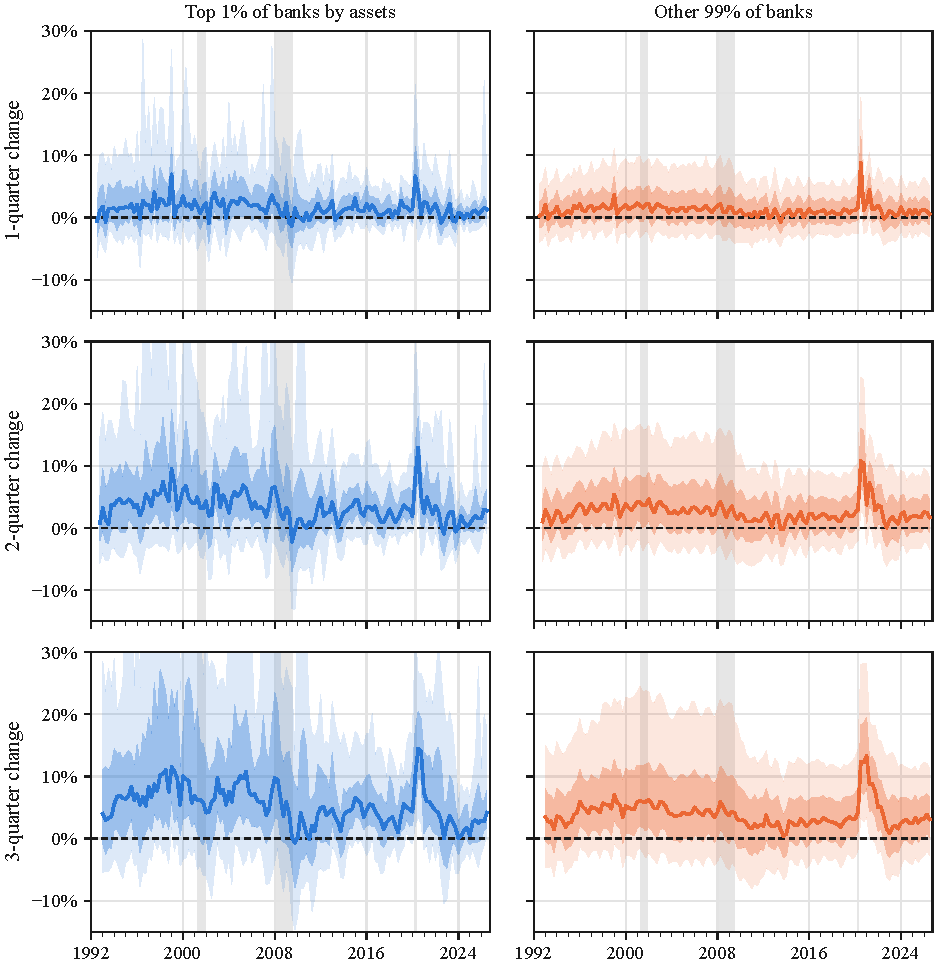
\includegraphics[width=\textwidth]{size_diff_assets_bare.pdf}
  \caption{Change in total assets (percent).}
  \label{fig:assets}
  \vspace{0.2em}
  \begin{minipage}{\textwidth}\footnotesize
    \textit{Notes:} Percent change in each bank's total assets from $k$ quarters earlier, including mergers and acquisitions. The vertical axis is capped at $-15\%$ and $30\%$. Line: median bank; dark band: 25th--75th percentiles; light band: 10th--90th percentiles. Shaded areas indicate NBER recessions. \textit{Source:} FDIC Statistics on Depository Institutions; author's calculations.
  \end{minipage}
\end{figure}

\begin{figure}[H]
  \centering
  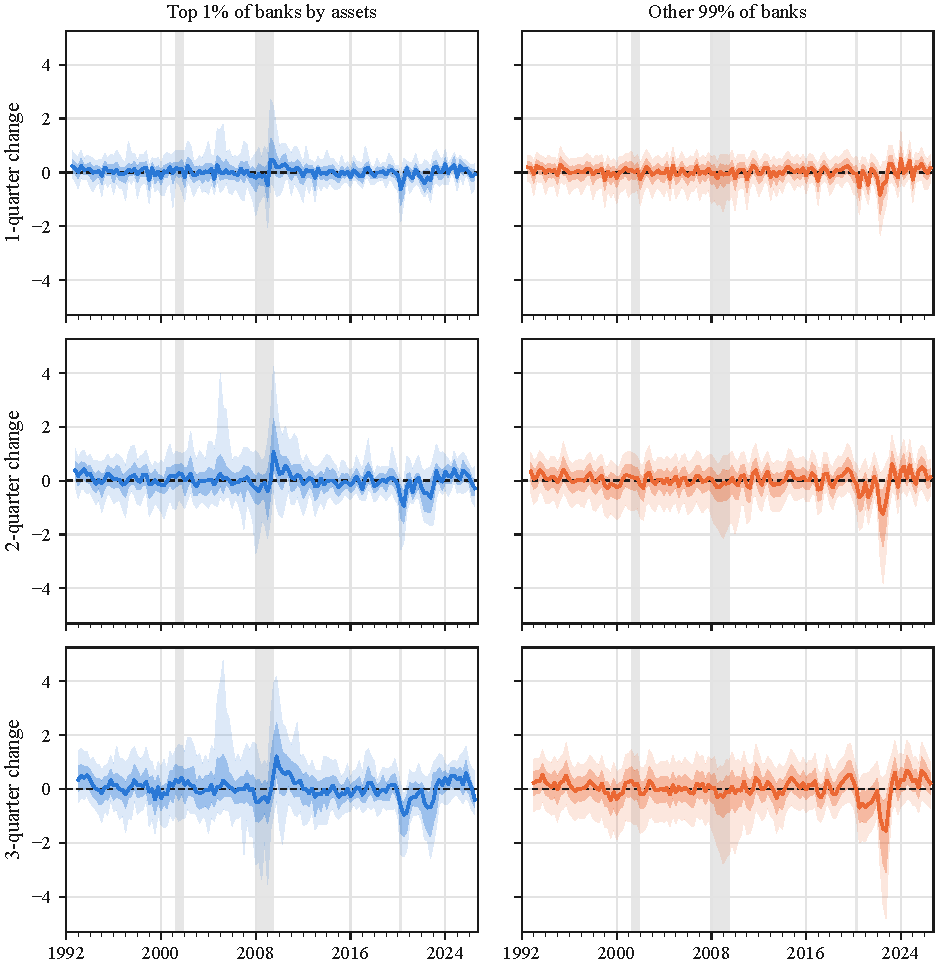
\includegraphics[width=\textwidth]{size_diff_equity_ratio_bare.pdf}
  \caption{Change in equity capital to assets (percentage points).}
  \label{fig:equity}
  \vspace{0.2em}
  \begin{minipage}{\textwidth}\footnotesize
    \textit{Notes:} Percentage-point change in each bank's equity-to-assets ratio from $k$ quarters earlier. Bands as in Figure~\ref{fig:assets}. \textit{Source:} FDIC Statistics on Depository Institutions; author's calculations.
  \end{minipage}
\end{figure}

\begin{figure}[H]
  \centering
  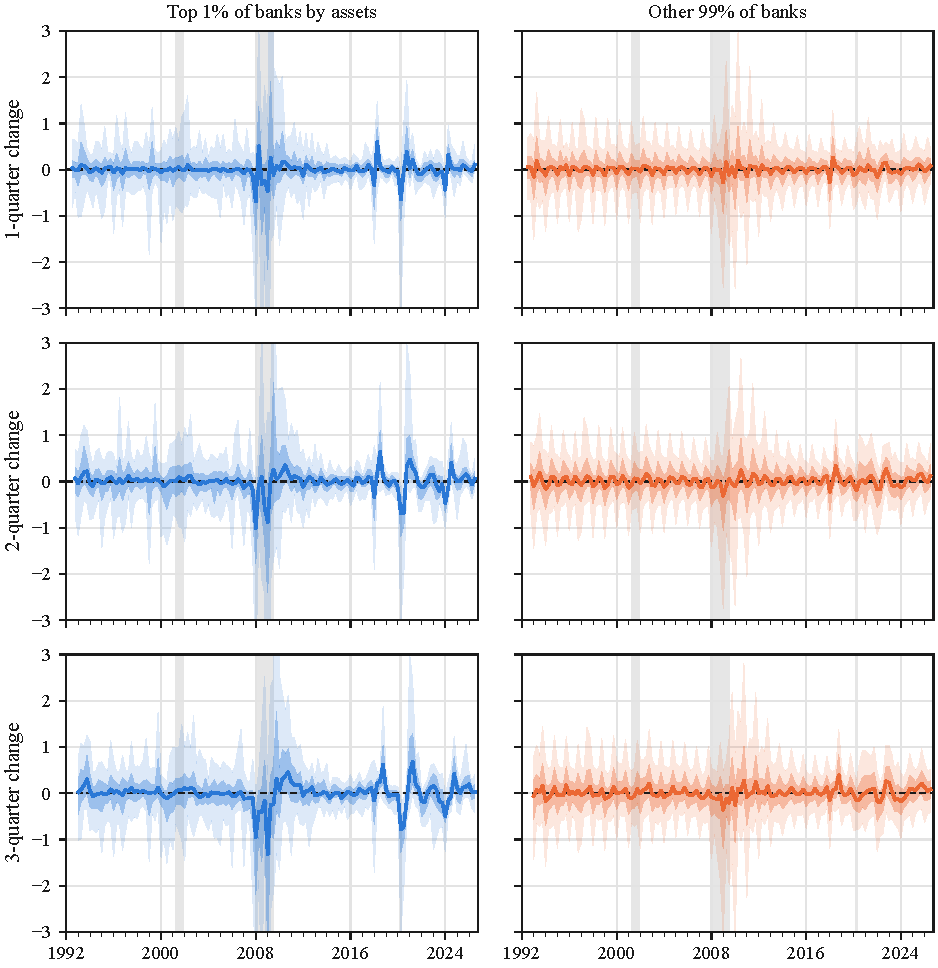
\includegraphics[width=\textwidth]{size_diff_roa_bare.pdf}
  \caption{Change in single-quarter return on assets (percentage points).}
  \label{fig:roa}
  \vspace{0.2em}
  \begin{minipage}{\textwidth}\footnotesize
    \textit{Notes:} Percentage-point change in each bank's single-quarter, annualized ROA from $k$ quarters earlier. The vertical axis is capped at $\pm 3$, which clips the large-bank tails in 2008--09. Bands as in Figure~\ref{fig:assets}. \textit{Source:} FDIC Statistics on Depository Institutions; author's calculations.
  \end{minipage}
\end{figure}

\begin{figure}[H]
  \centering
  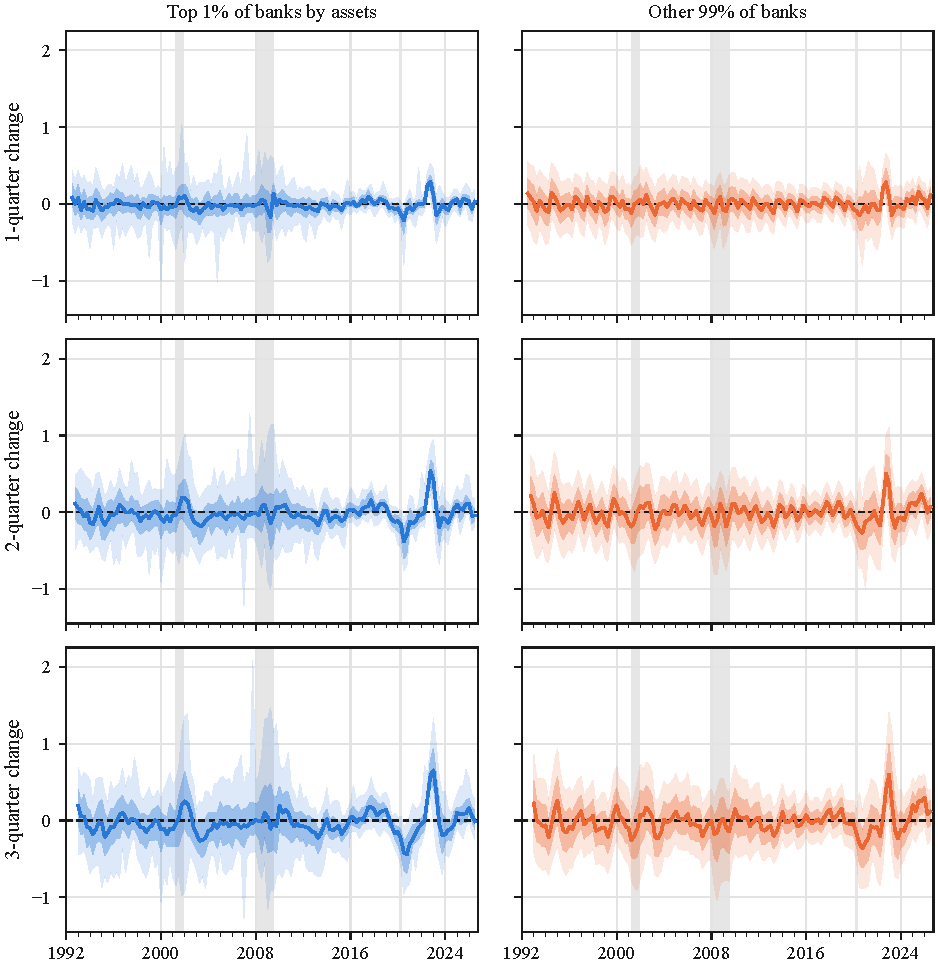
\includegraphics[width=\textwidth]{size_diff_nim_bare.pdf}
  \caption{Change in single-quarter net interest margin (percentage points).}
  \label{fig:nim}
  \vspace{0.2em}
  \begin{minipage}{\textwidth}\footnotesize
    \textit{Notes:} Percentage-point change in each bank's single-quarter, annualized NIM from $k$ quarters earlier. Bands as in Figure~\ref{fig:assets}. \textit{Source:} FDIC Statistics on Depository Institutions; author's calculations.
  \end{minipage}
\end{figure}

\begin{figure}[H]
  \centering
  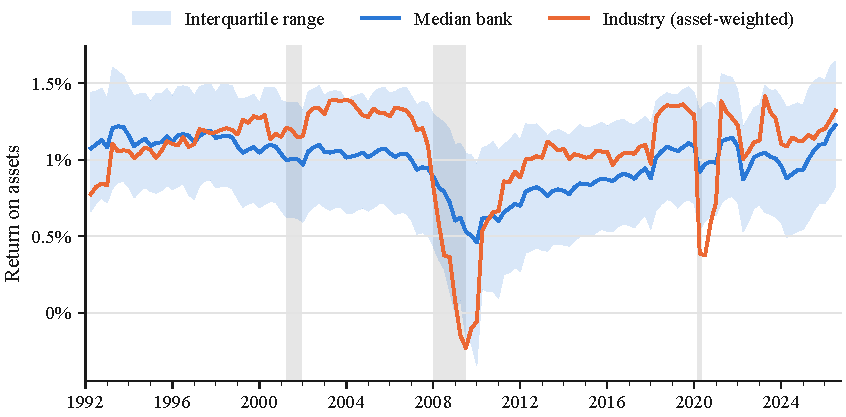
\includegraphics[width=\textwidth]{banks_roa_distribution_bare.pdf}
  \caption{Aggregate versus typical bank: return on assets.}
  \label{fig:roadist}
  \vspace{0.2em}
  \begin{minipage}{\textwidth}\footnotesize
    \textit{Notes:} Reported (year-to-date, annualized) ROA. The asset-weighted industry figure is dominated by the largest banks; the median and interquartile range describe the typical bank. Shaded areas indicate NBER recessions. \textit{Source:} FDIC Statistics on Depository Institutions; author's calculations.
  \end{minipage}
\end{figure}

\begin{figure}[H]
  \centering
  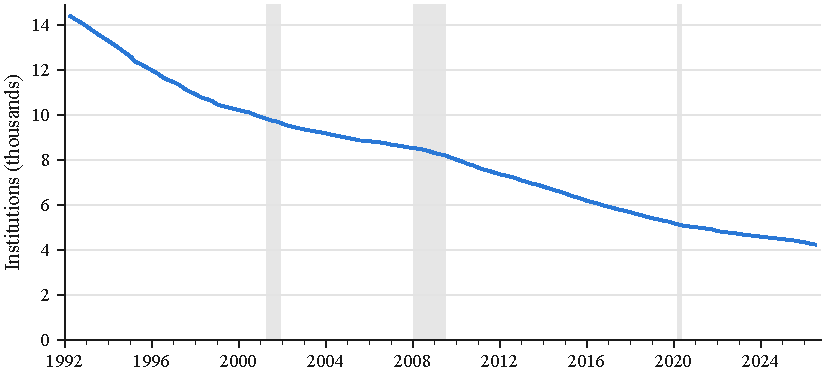
\includegraphics[width=\textwidth]{banks_count_bare.pdf}
  \caption{Number of FDIC-insured institutions filing a call report.}
  \label{fig:count}
  \vspace{0.2em}
  \begin{minipage}{\textwidth}\footnotesize
    \textit{Notes:} Excludes insured branches of foreign banks. Shaded areas indicate NBER recessions. \textit{Source:} FDIC Statistics on Depository Institutions; author's calculations.
  \end{minipage}
\end{figure}

\section*{Visual Findings}

\paragraph{Assets.}
Upon initial assessment, the different lags have similar distributions, just stretched out over the their tails. Additionally, the size of the upside tail for the top 1\% of banks is much larger than the other banks, though the median seems somewhat stable. Also, the smaller asset-sized group appears to have a more symmetric distribution over the time period. Looking particularly during recessions, the downside tail of the large banks is much more pronounced than the other banks, which is consistent with the idea that larger banks are more exposed to macroeconomic shocks. This also mirrors trends in household income distributions.

\paragraph{Equity ratio.}
As opposed to asset distributions, equity ratio distributions are more symmetric and stable over time, with the exception of the 2008--09 financial crisis and COVID-19 recession. Both have overwhelmingly downside tails during recessionary periods, and appear to be left-skewed even in expansionary periods. The actual median does appear to be same across groups and moves similarly.

\paragraph{ROA.} 
This measure appears to be the most volatile of the four, with the largest upside and downside tails. The large-bank group has a much more dense upside tail, especially during economic rebound periods. The furthest outliers of the majority of banks appears much more sparse. The sawtooth pattern of the right-hand group is likely due to the fact that ROA is annualized, and the first quarter of each year is compared to the fourth quarter of the previous year. 

\paragraph{NIM.} 
The net interest margin distributions appear the most stable of the four. The sawtooth pattern is again present due to the annualization. Distributions tend to be very tight to the median outside of recessionary periods. Overall, the effects seem to symmetric.

\section*{Potential Concerns}

\paragraph{Grouping on current size selects on growth.}
Because group membership is determined by assets at $t$, a bank that crossed into the top 1\% through rapid growth or an acquisition is, mechanically, a large bank with a large asset change. This inflates the upper tail and the right skew of large-bank asset growth, and to a lesser extent anything correlated with growth. A robustness check is to assign groups using assets at $t-k$, or to fix membership at the start of each episode.

\paragraph{Survivorship and entry.}
A change is defined only if the bank reports in both $t-k$ and $t$. Banks that fail or are absorbed drop out after their last filing, so the very worst outcomes, such as a bank's final quarter before closure, can be missing from the lower tail. New charters enter only after $k$ quarters. Both effects matter most in 2008--10, when a large number of institutions failed.

\paragraph{Small groups make tails noisy.}
The large-bank group contains 42--143 banks, so its 10th and 90th percentiles are set by roughly the 4th to 14th most extreme institution. This creates larger skewness artifically just by the small sample size, and it makes the tails of the large-bank distributions more volatile than those of the other-bank group. For the actual analysis, this will likely need to be extended significantly.

\paragraph{Few recession quarters, one dominant episode.}
Only 11 of 138 quarters overlap a recession, and 6 of them fall in 2008--09. The recession columns of the tables are therefore mostly a description of the financial crisis. The 2001 recession barely registers in the bank data, and the 2020 recession is only two quarters long and is confounded by pandemic-era deposit inflows and loan-loss provisioning. For this reason, finding someway to correlate the distributions with a macroeconomic indicator such as the unemployment rate or the federal funds rate may be more informative than a binary recession indicator. However, there is heavy endogeneity in the relationship between such otucomes and our data, so finding an exogenous measure or creating some limits on the predictive power of the macroeconomic indicator may be necessary.

\paragraph{Overlapping horizons and seasonality.}
It appears that distribtions generally move in the same way over the span of a year, so $t-1$, $t-2$, and $t-3$ are not independent. Particularly, it appears that abnormal changes in across a one quarter lag correlate to an even larger, same-signed change in the three quarter lag. 

\paragraph{Axis caps.}
The vertical axes of Figures~\ref{fig:assets} and~\ref{fig:roa} are truncated to keep the medians and inner bands legible.


\end{document}
